%!TEX root = ../presentation.tex


% -------------- BACKGROUNDS --------------

\newcommand\titlebackground {
    \usebackgroundtemplate{
    \begin{tikzpicture}[remember picture, overlay]
        \node[at=(current page.center)] {
            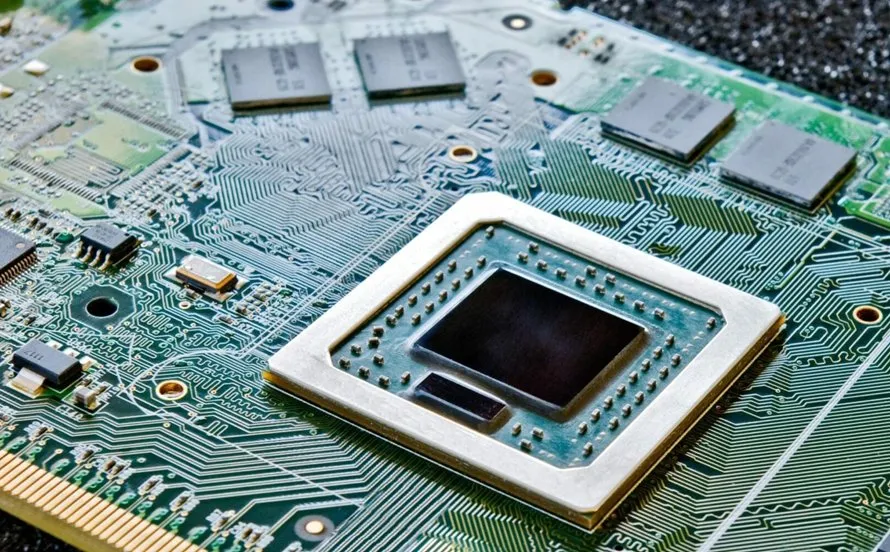
\includegraphics
            [width=\paperwidth, keepaspectratio]
            {pictures/background/background-PCB.png}
        };
    \end{tikzpicture}
    }
}


\newcommand\introbackground {
    \usebackgroundtemplate{
    \begin{tikzpicture}[remember picture, overlay]
        \node[at=(current page.center)] {
            
\includegraphics
            [width=\paperwidth, keepaspectratio]
            {pictures/background/background-pcb-poster.png}
        };
    \end{tikzpicture}
    }
}

\newcommand\defaultbackground {
    \usebackgroundtemplate{
    \begin{tikzpicture}[remember picture, overlay]
        \node[at=(current page.center)] {
            
\includegraphics
            [width=\paperwidth, keepaspectratio]
            {pictures/background/background5.pdf}
        };
    \end{tikzpicture}
    }
}


% -------------- TITLE PAGE --------------
\makeatletter
\newcommand\titlegraphicii[1]{\def\inserttitlegraphicii{#1}}
\titlegraphicii{}
\setbeamertemplate{title page}
{
    {
        \usebeamercolor[fg]{titlegraphic}
        \inserttitlegraphic\hfill\inserttitlegraphicii
        \\
    }

    \begin{multicols}{2}
        \begin{beamercolorbox}[sep=8pt, center, shadow=true, rounded=true, wd=0.5\textwidth, bgopacity=0.85]{title}
            \usebeamerfont{title}
            \textbf{\inserttitle}\\
            {
                \usebeamerfont{subtitle}\usebeamercolor[fg]{subtitle}
                \textbf{\insertsubtitle}\\
            }
            {
                \vspace{24pt}
                \small\usebeamerfont{author}
                \insertauthor\\
            }
        \end{beamercolorbox}
    \vfill\null
    \columnbreak
    \end{multicols}
}
\makeatother


\newcommand\thankyouframe{
    \begin{frame}
    \begin{multicols}{2}
        \begin{beamercolorbox}[sep=8pt, center, shadow=true, rounded=true, wd=0.5\textwidth, bgopacity=0.85]{title}
            \usebeamerfont{title}Merci!\\
        \end{beamercolorbox}%
    \vfill\null
    \columnbreak
    \end{multicols}
\end{frame}
}
